\section{Практична частина}
\setlength{\parindent}{4em}

\begin{center}
  {\textbf{\emph{Визначення глубини}}}
\end{center}
\begin{figure}[ht]

\centering

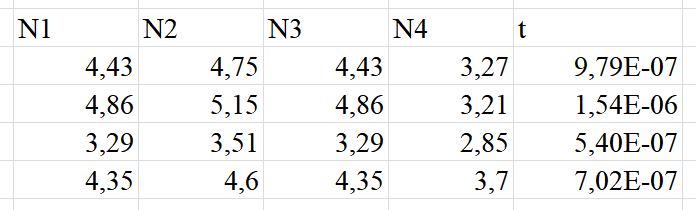
\includegraphics[width=0.55\linewidth]{Pics/table1.png}


\label{Teo}

\end{figure}
У данній лабораторній роботі ми визначали змінну, що не має певного значення, тому ми не можемо визначити теоретичне відхилення, чи порівняти з теоретичним значенням.
